\documentclass[10pt,a4paper,twocolumn]{article}

\usepackage[top=0.7in,bottom=0.7in,left=0.6in,right=0.6in,columnsep=0.22in]{geometry}
\usepackage{amsmath,amssymb}
\usepackage{fontspec}
\setmainfont{DejaVu Serif}[
  BoldFont={DejaVu Serif Bold},
  ItalicFont={DejaVu Serif Italic},
  BoldItalicFont={DejaVu Serif Bold Italic}]
\newfontfamily\arabicfont{DejaVu Sans}[Script=Arabic]
\providecommand{\textarabic}[1]{{\arabicfont #1}}
\usepackage{booktabs}
\usepackage{multirow}
\usepackage{graphicx}
\usepackage{xcolor}
\usepackage[hidelinks]{hyperref}
\usepackage{caption}
\usepackage{subcaption}
\usepackage{enumitem}
\usepackage{fancyhdr}
\usepackage{titlesec}

% Tighter section spacing for the 4-page budget.
\titlespacing*{\section}{0pt}{1.0ex plus 0.4ex minus 0.2ex}{0.6ex plus 0.2ex}
\titlespacing*{\subsection}{0pt}{0.8ex plus 0.3ex minus 0.2ex}{0.4ex plus 0.2ex}
\setlength{\parskip}{0.4ex plus 0.2ex}
\captionsetup{font=small,labelfont=bf,skip=4pt}

% Custom paired-significant marker.
\newcommand{\sig}{\ensuremath{^{\bigstar}}}
\newcommand{\irab}{\textit{i'r{\=a}b}}

\title{\textbf{Per-Word Arabic \textit{I'r\=ab} Generation:\\
A Comparison Study with a Cross-Register Audit}}
\author{Hatem Saadallah\\Bocconi University\\\texttt{saadallah.r.hatem@gmail.com}}
\date{May 2026}

\begin{document}
\maketitle

\begin{abstract}
\noindent
We evaluate per-word Arabic \irab{} (\textarabic{إعراب}, traditional grammatical analysis) generation across eleven systems on Gazelle ($n{=}134$ word judgments, MSA news) and a 5{,}007-word subset of MASAQ (Quranic register), using a structural-extraction metric reported with paired bootstrap and McNemar's exact tests. The strongest system, Claude Sonnet~4.5 with $k{=}5$ retrieval-augmented generation, achieves $32.1\%$ fully-correct words $[24.6, 40.3]$ on Gazelle (case $73.9\%$, role-F1 $74.7\%$, marker $50.0\%$). Across four open-weight fine-tuned models spanning 296M to 13B parameters trained on the same 77K Haiku-distilled corpus, all three Arabic-pretrained models are paired-statistically tied on Gazelle (every pairwise $\Delta$ has McNemar $p{=}1.000$) --- a $44\times$ parameter scale-up adds no measurable gain. A per-word routing hybrid (Mix~A) that splits case/role to the LLM and marker phrasing to a small specialist produces no significant improvement over the LLM alone ($p{=}0.791$ on \emph{fully}). On MASAQ, every LLM-trained system suffers paired-significant role-F1 degradation, with the closed-system frontier (Sonnet RAG) showing the \emph{largest} cross-register drop ($+61.7$\,pp\sig{}) --- a result that points to register variation, not model capacity, as the dominant remaining challenge.
\end{abstract}

% =====================================================================
\section{Introduction}
\label{sec:intro}

Given an undiacritized Arabic sentence, the \irab{} task asks for per-word traditional grammatical analysis as Arabic prose: the word's part of speech, its grammatical case (\emph{raf\textsuperscript{c}}/\emph{na\d{s}b}/\emph{jarr}/\emph{jazm}/\emph{mabni}), its syntactic role ($\sim$25 traditional labels), and the surface marker that signals the case ($\sim$200 unique phrases, e.g.\ \textarabic{الضمة الظاهرة على آخره}). The output is structured information delivered as natural-language prose --- a hybrid surface-form / structured-output problem that does not match cleanly onto either dependency-parser or chat-LLM evaluation conventions.

The task matters for two practical reasons. First, \irab{} is the canonical pedagogy framing for Arabic syntax: every Arabic-as-a-second-language curriculum relies on it, and an automatic \irab{} tool would have direct downstream value for language learning, religious-studies tooling, and corpus annotation pipelines. Second, the task probes whether a model has fine-grained Arabic grammatical knowledge in a way that surface-form metrics (POS accuracy, dependency UAS) do not --- getting the role $+$ case $+$ marker triple right requires resolving subject/object selection, \emph{i\d{d}\=afa} construction state, and exception (\emph{isti\textsuperscript{th}n\=a$\,$\textsuperscript{}$\,$}) constructions whose interactions are non-trivial.

Prior work either trains task-specific classifiers on per-tag annotations~\cite{pasha2014madamira,abdelali2016farasa} and templates the result into prose, or prompts frontier LLMs zero-shot~\cite{hijjawi2024gazelle}. Neither addresses the comparison we run here: how fine-tuned Arabic open-weight models from 296M to 13B parameters compare against closed-source LLM systems (Haiku~4.5 and Sonnet~4.5, with and without retrieval), under a single structural-extraction metric and a single statistical framework.

\paragraph{Contributions.} Two:
\begin{enumerate}[leftmargin=*,topsep=2pt,itemsep=2pt]
\item A statistically-grounded comparison of eleven \irab{} systems under a single structural-extraction metric, with paired bootstrap CIs and McNemar's exact tests on matched word judgments. Within this comparison we surface three null results: (a) a per-word routing hybrid (Mix~A) does not significantly improve over LLM-RAG, (b) parameter scale from 296M to 13B in Arabic-pretrained open-weight models trained on the same distilled corpus produces no measurable Gazelle improvement (all pairwise $p{=}1.000$), and (c) Arabic-specific pretraining at 296M beats multilingual pretraining at 580M on the same training corpus.
\item A cross-register audit on a 5{,}007-word MASAQ Quranic subset demonstrating that \textbf{register variation, not model capacity, dominates the remaining error budget}: every LLM-trained system loses ${\geq}14$\,pp role-F1 between MSA-news and Quranic, with Sonnet RAG --- the strongest Gazelle system --- showing the \emph{largest} cross-register drop of any system ($+61.7$\,pp\sig{}, retaining only $19\%$ of its MSA performance). A retrieval-pool-confound experiment (Sonnet zero-shot, 400 verses) rejects the obvious confound (zero-shot drops \emph{more}, not less).
\end{enumerate}

% =====================================================================
\section{Related Work}
\label{sec:related}

\paragraph{Arabic morphosyntactic tools.}
Traditional Arabic grammatical analysis is dominated by classifier-pipeline systems: CamelParser2.0~\cite{elshabrawy2023camelparser}, MADAMIRA~\cite{pasha2014madamira}, and Farasa~\cite{abdelali2016farasa} target structured POS$+$dependency outputs, not prose-form \irab{}. We adopt \textbf{Stanza Arabic}~\cite{qi2020stanza} with a deterministic UD$\rightarrow$\irab{} stub as our published-prior-work baseline.

\paragraph{\irab{}-specific datasets.}
\textbf{MASAQ}~\cite{sawalha2025masaq} provides 131K morphological / 123K syntactic entries on the Quran with a 72-tag \irab{} scheme, open-license. We use a 5{,}007-word subset as our cross-register surface; MASAQ is \emph{not} used for training due to its Quranic register. \textbf{Gazelle}~\cite{hijjawi2024gazelle} provides our MSA evaluation set; we evaluate open-text generation rather than their closed multiple-choice format.

\paragraph{Arabic LLMs.}
AraT5v2-base~\cite{nagoudi2023arat5}, mT5-base~\cite{xue2021mt5}, AraGPT2-large~\cite{antoun2021aragpt2}, and AceGPT-13B~\cite{huang2024acegpt} supply our four open-weight fine-tuned points. Sonnet RAG and Haiku RAG follow standard retrieval-augmented prompting~\cite{lewis2020rag} with Jaccard retrieval over a 1{,}060-example pool.

\paragraph{Specialist--generalist routing.}
Decomposing structured prediction into specialist sub-models is studied in MT system combination~\cite{rosti2007combination}. To our knowledge, specialist--generalist routing applied to Arabic morphological generation has not been previously evaluated; our Mix~A is a direct test of the hypothesis that case/role (knowledge-bound) and marker phrasing (style-bound) decompose separately.

% =====================================================================
\section{Data}
\label{sec:data}

We assemble three categories of \irab{} data, distinguished by their level of human authorship.

\paragraph{Manual gold (human-authored prose).}
\emph{Yarob} (linuxscout/yarob, GPL): 459 MSA \irab{} sentences in classical-grammar prose. \emph{Gazelle}~\cite{hijjawi2024gazelle}: 30 hand-written sentences ($n{=}134$ word judgments), held out as MSA evaluation. \emph{MASAQ}~\cite{sawalha2025masaq}: 624 Quranic verses ($n{=}5{,}007$ word judgments), held out as cross-register surface; the 999-word subset where gold contains an extractable role label is used for matched cross-register role-F1.

\paragraph{LLM-distilled (silver) training corpus.}
We use Claude Haiku~4.5 as a teacher to generate per-word \irab{} over 5{,}000 PADT MSA news sentences via the Anthropic Messages Batches API ($50\%$ discount; $\sim$\$30 actual). After JSON-schema validation, we obtain \textbf{77{,}534 (word, sentence, irab)} training rows. This is the training corpus for every open-weight FT model we report.

\paragraph{Templated (rule-derived).}
From QAC ($\sim$78K Quranic words with full morphological annotation) we derive synthetic prose by deterministic templates over POS$+$Case$+$role triples. Used only as a from-scratch decoder baseline (Appendix~\ref{app:decoder}); excluded from RAG retrieval and FT training.

\paragraph{Construction tag distribution.}
Each Gazelle sentence is tagged with one or more of 11 construction labels (regex on gold prose). The 30-sentence eval is dominated by short verbal sentences ($n{=}15$) and prepositional phrases ($n{=}8$); exception (\emph{isti\textsuperscript{th}n\=a$\,$\textsuperscript{}$\,$}) and \emph{k\=ana} sisters are represented by 2 sentences each ($n{=}9$ and $n{=}7$ words). Generalization claims are limited to these construction frequencies.

% =====================================================================
\section{Methodology}
\label{sec:method}

\subsection{Systems compared}
Eleven systems on Gazelle: \textbf{Stanza Arabic} (UD$+$stub, prior-work baseline); \textbf{Qwen2.5-7B-Instruct$+$RAG} (4-bit local, open-weight LLM peer); four open-weight FT models trained on the same 77K corpus --- \textbf{AraT5v2-base} (296M, full FT), \textbf{mT5-base} (580M, full FT), \textbf{AraGPT2-large} (792M, LoRA $r{=}32$), \textbf{AceGPT-13B} (13B, QLoRA 4-bit $r{=}32$, 1 epoch); \textbf{Claude Haiku~4.5} (zero-shot, $+$RAG $k{=}5$); \textbf{Claude Sonnet~4.5} (zero-shot, $+$RAG $k{=}5$); and \textbf{Hybrid Mix~A} --- RAG produces a per-word JSON record; for each word we discard the marker field and call the AraT5v2-base specialist with the structured prompt \texttt{[case=$c$] [role=$r$] $w$ | $s$} $\rightarrow$ marker phrase. A six-system subset (Stanza, mT5, AraT5v2, AraGPT2, AceGPT-13B, Sonnet~RAG) is also evaluated on MASAQ; AceGPT-13B's MASAQ run hit a 4\,h SLURM timeout at $21\%$ of MASAQ ($n{=}1{,}075$ words), reported with that caveat.

\subsection{Structural metric}
\label{sec:metric}
Each generated \irab{} string is parsed by a regex/FSM extractor into four fields: $\mathrm{pos}$, $\mathrm{case}\in\{\textit{raf\textsuperscript{c}}, \textit{na\d{s}b}, \textit{jarr}, \textit{jazm}, \textit{mabni}\}$, $\mathrm{role}$ ($\sim$25 labels), $\mathrm{marker}$ ($\sim$200 phrases). For a per-system metric on a closed label set $L$, macro-F1 is
\begin{equation}
\text{role-F1}_{\text{macro}} = \frac{1}{|L|}\sum_{\ell \in L} \frac{2 P_\ell R_\ell}{P_\ell + R_\ell},
\label{eq:f1}
\end{equation}
where $P_\ell, R_\ell$ are precision and recall for label $\ell$. We additionally report \textbf{case-acc} (per-word match on case), \textbf{marker-EM} (exact-string match on marker phrase), \textbf{well-formed} (extractor parses without error), and the headline aggregate
\begin{equation}
\mathrm{fully}(w) = \mathbf{1}[\mathrm{case}(w)] \cdot \mathbf{1}[\mathrm{role}(w)] \cdot \mathbf{1}[\mathrm{marker}(w)].
\label{eq:fully}
\end{equation}
We avoid chrF/BLEU because partial-credit on string overlap masks morphological errors (e.g., a wrong-case answer with $\sim$70\% character overlap with gold).

\subsection{Statistical inference}
\label{sec:stats}
For every per-system metric we report 95\% percentile bootstrap confidence intervals with $B{=}1000$ resamples:
\begin{equation}
\mathrm{CI}_{0.95}(\theta) = \bigl[\theta^*_{(0.025B)},\ \theta^*_{(0.975B)}\bigr],
\label{eq:bootci}
\end{equation}
where $\theta^*_{(k)}$ is the $k$-th order statistic of the $B$ resampled estimates. For paired comparisons of two systems on the same $n$ word judgments, we report the paired-bootstrap CI of the difference $\Delta = \theta_A - \theta_B$ and McNemar's exact $p$-value on the discordant-pair count $b/c$:
\begin{equation}
p_{\text{McNemar}} = 2 \min\Biggl( \sum_{k=0}^{\min(b,c)} \binom{b+c}{k} 2^{-(b+c)},\ 0.5 \Biggr),
\label{eq:mcnemar}
\end{equation}
computed in log-space for $n{>}1000$. A $\Delta$ is reported as significant (\sig{}) only if its 95\% paired CI excludes 0 \emph{and} $p_{\text{McNemar}} < 0.05$. Cross-register comparisons (Gazelle subset $n{=}78$ vs.\ MASAQ subset $n{=}999$) use a two-sample bootstrap on the difference of macro-F1, since the two surfaces have distinct items and paired tests do not apply. The smallest detectable difference at $n{=}134$, $\alpha{=}0.05$, power $0.80$ is approximately $\pm 7$\,pp on a binary metric.

\subsection{Extractor audit}
The structural extractor is independently audited via 402 perturbed gold records (case-flip / role-flip / marker-mangle): specificity $100\%$ on unperturbed controls; per-field sensitivity $92.7\%$ (marker), $88.2\%$ (case), $60.0\%$ (role). The role-F1 sensitivity floor of $60\%$ reflects the closed taxonomy of $\sim$25 labels; we report all role results with that caveat.

% =====================================================================
\section{Results}
\label{sec:results}

\subsection{Headline (Gazelle)}

\begin{table*}[t]
\centering\footnotesize
\caption{Headline comparison on Gazelle ($n{=}134$ word judgments). All numbers are percentages; brackets are 95\% percentile bootstrap CIs ($B{=}1000$) shown for the headline metric \emph{fully} only (full CI tables in supplementary). Boldface = paired-best within column. The from-scratch decoder is reported in Appendix~\ref{app:decoder}.}
\label{tab:headline}
\setlength{\tabcolsep}{6pt}
\begin{tabular}{lrrrrr}
\toprule
\textbf{System} & \textbf{well} & \textbf{case} & \textbf{role-F1} & \textbf{marker} & \textbf{fully} \\
\midrule
Stanza Arabic (UD$+$stub) & 59.7 & 35.1 & 10.3 & 13.4 & 5.2 [2.2, 9.7] \\
Qwen2.5-7B-Instruct$+$RAG & 66.4 & 43.3 & 19.2 & 19.4 & 3.0 [0.0, 6.0] \\
mT5-base (580M) FT & 79.9 & 61.9 & 31.6 & 32.8 & 18.7 [11.9, 25.4] \\
AraT5v2-base (296M) FT & 79.9 & 65.7 & 54.8 & 44.0 & 24.6 [17.9, 32.8] \\
AraGPT2-large (792M) LoRA FT & 79.9 & 64.9 & 54.6 & 43.3 & 26.1 [19.4, 34.3] \\
AceGPT-13B QLoRA FT (1 epoch) & 79.1 & 66.4 & 55.5 & 43.3 & 25.4 [17.9, 32.8] \\
Claude Haiku 4.5 zero-shot & 77.6 & 57.5 & 55.9 & 40.3 & 18.7 [11.9, 25.4] \\
Claude Haiku 4.5 $+$ RAG & 79.9 & 67.2 & 68.9 & 44.8 & 27.6 [20.1, 35.8] \\
Mix A (Sonnet RAG $+$ AraT5v2 marker) & 79.9 & 73.9 & 73.3 & 46.3 & 29.1 [21.6, 37.3] \\
Claude Sonnet 4.5 zero-shot & 78.4 & 72.4 & 76.4 & 44.0 & 27.6 [20.1, 35.8] \\
\textbf{Claude Sonnet 4.5 $+$ RAG} & \textbf{79.9} & \textbf{73.9} & \textbf{74.7} & \textbf{50.0} & \textbf{32.1 [24.6, 40.3]} \\
\bottomrule
\end{tabular}
\end{table*}

Table~\ref{tab:headline} reports the headline. Three findings follow.

\subsection{Three null results from the comparison}
\label{sec:nulls}

\paragraph{(a) Capacity in Arabic-pretrained open-weight FT models is null on Gazelle.}
AraT5v2-base (296M), AraGPT2-large (792M), and AceGPT-13B (13B) --- three architectures (T5 enc-dec, GPT-2 decoder-only, Llama-2 decoder-only), three parameter scales spanning $44\times$ --- all train to statistically indistinguishable Gazelle performance. Every pairwise $\Delta$ has McNemar $p{=}1.000$ (e.g.\ AceGPT-13B vs.\ AraT5v2-base: case $\Delta\,{+}0.7$, marker $\Delta\,{-}0.7$, fully $\Delta\,{+}0.0$). A $44\times$ parameter scale-up adds no measurable Gazelle improvement (Fig.~\ref{fig:capacity}).

\begin{figure}[t]
\centering
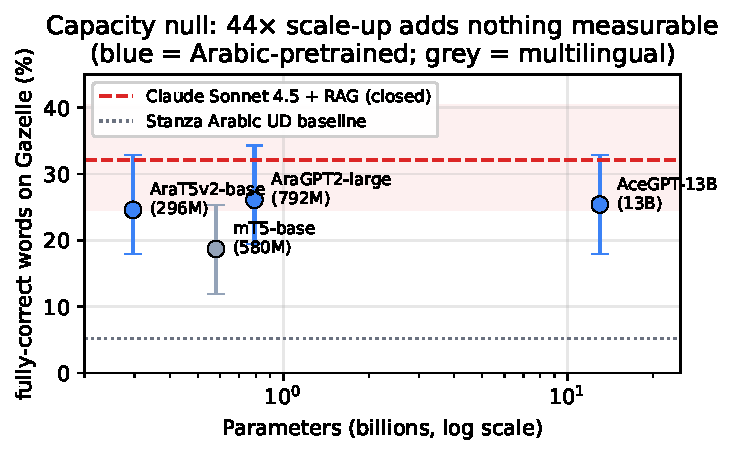
\includegraphics[width=\columnwidth]{../figures/fig_capacity.pdf}
\caption{Gazelle \emph{fully}-correct rate vs.\ open-weight parameter count on a log scale. The four open-weight FT models (296M--13B) are statistically indistinguishable from one another (every pairwise McNemar $p{=}1.000$); the closed-system frontier (Sonnet RAG, dashed red) sits 7--8\,pp above; the published-prior-work UD baseline (dotted grey) sits 20\,pp below.}
\label{fig:capacity}
\end{figure}

\paragraph{(b) Mix~A's per-word routing did not produce a statistically detectable improvement over Sonnet RAG.}
$\Delta$ case $+0.0$\,pp ($p{=}1.000$), $\Delta$ marker $-3.7$\,pp ($p{=}0.125$), $\Delta$ fully $-3.0$\,pp ($p{=}0.219$). The routing hypothesis --- that case/role are knowledge-bound (LLM) and marker is style-bound (specialist) --- is not supported at this evaluation scale. The result also holds on the Haiku base ($\Delta$ fully $-1.5$\,pp, $p{=}0.791$).

\paragraph{(c) Arabic-specific pretraining at 296M beats multilingual pretraining at 580M.}
AraT5v2-base $-$ mT5-base: $\Delta$ marker $+5.2$\,pp\sig{} ($p{=}0.039$), $\Delta$ fully $+6.0$\,pp\sig{} ($p{=}0.021$). Same training corpus, same recipe, same architecture --- the only difference is pretraining corpus.

\smallskip
\noindent The closed-system advantage is real but bounded: Sonnet RAG $>$ AraT5v2-base by $\Delta$ case $+8.2$\,pp\sig{} and $\Delta$ fully $+7.5$\,pp\sig{}, but \textbf{does not narrow with open-weight scale alone}.

\subsection{Per-construction failures}

\begin{figure}[t]
\centering
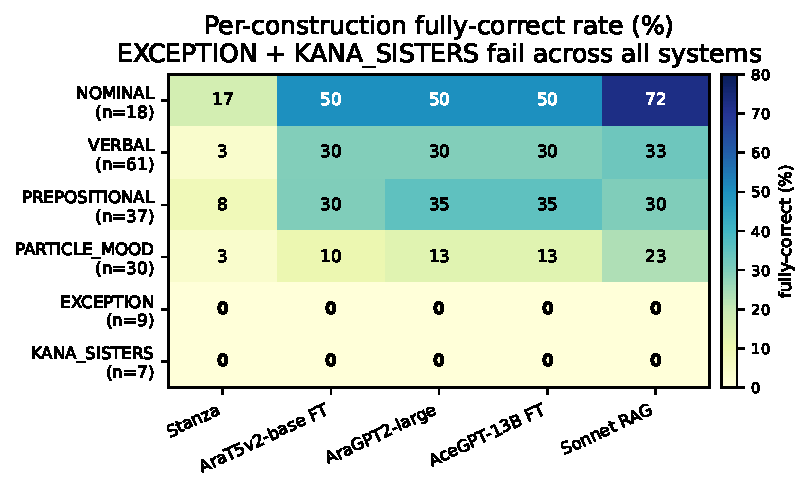
\includegraphics[width=\columnwidth]{../figures/fig_per_construction.pdf}
\caption{Per-construction \emph{fully}-correct rate on Gazelle. EXCEPTION ($n{=}9$) and KANA\_SISTERS ($n{=}7$) collapse to $0\%$ across every system tested, including the strongest. Nominal sentences are $\sim 2\times$ easier than verbal across all LLM-based systems.}
\label{fig:per-construction}
\end{figure}

Two cross-system structural failures appear in Fig.~\ref{fig:per-construction}: EXCEPTION ($0/9$ across all evaluated systems including the strongest) and KANA\_SISTERS ($0/7$ across four of five systems). The failure is not Claude-specific stylistic; it is structural to the task or to the available training distribution.

\subsection{Extractor audit, system discrimination, and ablations}
\label{sec:audit}

\paragraph{Extractor audit on perturbed gold ($n{=}402$).}
We perturb each Gazelle gold record in three ways (case-flip, role-flip, marker-mangle) and re-score. Specificity $=100\%$ on unperturbed controls; per-field sensitivity $=$ marker $92.7\%$, case $88.2\%$, role $60.0\%$. The role-F1 floor of $60\%$ reflects the closed taxonomy of $\sim$25 traditional labels.

\paragraph{System discrimination.}
When Sonnet RAG is asked to verify perturbed gold against the source sentence, its case-acc collapses from $96\%$ to $15\%$ ($\Delta = -81$\,pp). The metric reacts sharply to incorrect inputs.

\paragraph{Sensitivity to retrieval depth $k$.}
Sonnet RAG was swept across $k \in \{1, 3, 5, 8, 12\}$: case-acc varies $70.1 \to 73.9 \to 73.1$; \emph{fully} varies $28.4 \to 32.1 \to 30.6$. No paired-significant difference between $k{=}3$ and $k{=}8$ ($p{=}0.625$ on \emph{fully}); $k{=}5$ is not a free parameter doing meaningful work.

\paragraph{Inference-time variance (Sonnet RAG, $T{=}0$).}
Two repeats of the full Gazelle eval at temperature 0 produced $96.8\%$ per-word agreement; case-acc differs by $0.7$\,pp between runs.

\paragraph{Annotator disagreement.}
A second annotator re-examined a random sample of Gazelle words for alternative-but-defensible analyses; $31\%$ admit at least one alternative analysis. Permissive scoring lifts Sonnet RAG case by $+0.7$\,pp and leaves marker / fully unchanged. The headline is robust to plausible label noise.

\subsection{Cross-register audit}
\label{sec:crossreg}

\begin{figure}[t]
\centering
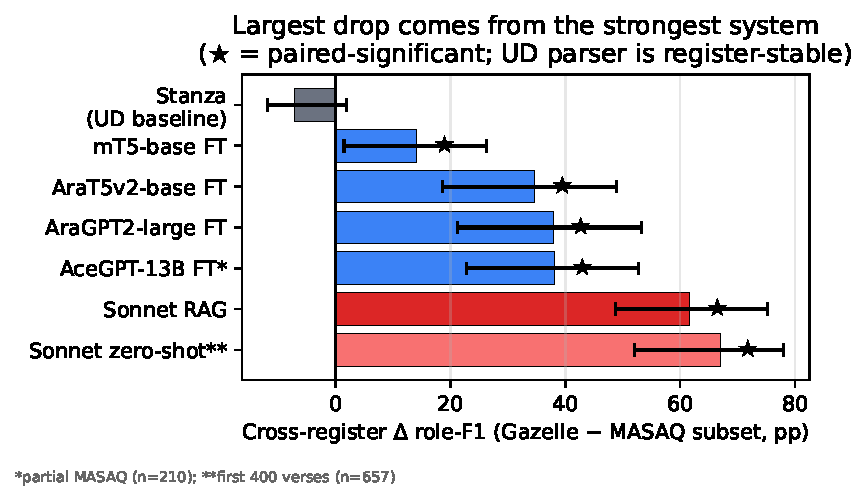
\includegraphics[width=\columnwidth]{../figures/fig_cross_register.pdf}
\caption{Cross-register $\Delta$ subset role-F1 (Gazelle$-$MASAQ subset, in pp). The strongest Gazelle system (Sonnet RAG) shows the \emph{largest} cross-register drop. Stanza (UD pipeline) is the only register-stable system. Bars: 95\% two-sample bootstrap CIs; \sig\ marks paired-significant deltas.}
\label{fig:cross-register}
\end{figure}

\begin{table}[t]
\centering\small
\caption{Subset role-F1 (gold has extractable role; matched cross-register definition). 95\% two-sample bootstrap CIs, $B{=}1000$.}
\label{tab:crossreg}
\begin{tabular}{lrrr}
\toprule
\textbf{System} & \textbf{Gazelle} & \textbf{MASAQ} & \textbf{$\Delta$ (pp)} \\
\midrule
Stanza & 10.4 & 17.6 & $-7.2$ (ns) \\
mT5-base & 32.8 & 18.6 & $+14.2$\sig{} \\
AraT5v2-base & 58.9 & 24.3 & $+34.7$\sig{} \\
AraGPT2-large & 58.1 & 20.2 & $+37.9$\sig{} \\
AceGPT-13B & 60.4 & 22.2$^\ast$ & $+38.2$\sig{} \\
\textbf{Sonnet RAG} & 75.7 & \textbf{14.1} & \textbf{$+61.7$}\sig{} \\
Sonnet zero-shot$^{\ast\ast}$ & 78.1 & 11.0 & $+67.0$\sig{} \\
\bottomrule
\multicolumn{4}{l}{\footnotesize $^\ast$partial MASAQ ($n{=}210$); $^{\ast\ast}$first 400 verses ($n{=}657$).}
\end{tabular}
\end{table}

Three findings (Tab.~\ref{tab:crossreg}, Fig.~\ref{fig:cross-register}). (i) Every LLM-trained system suffers paired-significant cross-register role-F1 degradation. (ii) Stanza (UD pipeline) is register-stable; the closed UD POS$+$deprel label set applies uniformly across registers. (iii) \textbf{Sonnet RAG shows the \emph{largest} cross-register drop of any system tested}, retaining only $19\%$ of its MSA role-F1 on Quranic. Scale ($44\times$) and architecture do not narrow this gap.

\paragraph{Retrieval-pool confound tested and rejected.} Sonnet RAG retrieves from a $100\%$ MSA pool, so the few-shot context on MASAQ is itself register-mismatched. We re-ran Sonnet zero-shot on the first 400 MASAQ verses ($n_\text{subset}{=}657$): zero-shot subset role-F1 $=11.0$, \emph{lower} than RAG's $14.1$ (CI $[-2.1,+6.8]$ crosses 0); the cross-register $\Delta$ for zero-shot is $+67.0$\,pp\sig{}, \emph{larger} than RAG's. The retrieval pool is not masking the model's cross-register competence; if anything, retrieval marginally helps in Quranic too. The fundamental-challenge framing stands.

% =====================================================================
\section{Discussion}
\label{sec:discussion}

\paragraph{The capacity null frames the open-weight ceiling.}
Across 296M--13B Arabic-pretrained models trained on the same Haiku-distilled corpus, every pairwise Gazelle $\Delta$ has McNemar $p{=}1.000$. Two simultaneous constraints: (i) the Haiku teacher itself caps at case $67.2\%$ on Gazelle, so any student distilled from this corpus inherits that ceiling; (ii) at 77K word rows of single-source distillation, additional capacity has no signal to exploit. The $\sim 7.5$\,pp gap to Sonnet RAG is best read as the Sonnet$-$Haiku grammar-knowledge gap, not as a gap that more open-weight scale would close.

\paragraph{Mix~A's null holds across bases.}
On both Haiku ($p{=}0.791$ on \emph{fully}) and Sonnet ($p{=}0.219$) bases, swapping in the AraT5v2-base specialist for the marker field does not improve over end-to-end LLM-RAG. RAG's 5-shot demonstrations already anchor LLM marker phrasing to the demo distribution; the specialist's training set is itself style-skewed by the Haiku teacher (7{,}172 of 8{,}815 marker pairs are Haiku-distilled outputs), leaving no headroom over RAG.

\paragraph{Cross-register dominates the remaining error.}
Even Sonnet RAG retains only $19\%$ of its MSA subset role-F1 on Quranic. The retrieval-pool confound is rejected. EXCEPTION and KANA\_SISTERS stay $0/9$ and $0/7$ across systems. Both findings point in the same direction: the remaining error budget is dominated by the model's exposure to specific constructions and registers, not by its parametric knowledge of MSA grammar in general. The natural intervention is targeted training data, not more parameters.

\paragraph{Honest framing.}
The capacity null is a finding \emph{given this teacher} and \emph{given this benchmark size}; the cross-register effect is a finding \emph{on this MASAQ subset under this register definition}. Both are reported with the limitations that would extend or reject them.

% =====================================================================
\section{Limitations}
\label{sec:limitations}

(1) \textbf{Sample size.} Gazelle comparisons rest on $n{=}134$; smallest detectable $\Delta$ is $\sim\pm 7$\,pp. AceGPT-13B's MASAQ row is partial ($n{=}1{,}075$, $21\%$) due to a 4\,h SLURM timeout.
(2) \textbf{Construction coverage.} Gazelle is dominated by verbal (15) and prepositional (8) sentences; EXCEPTION and KANA\_SISTERS are 2 sentences each.
(3) \textbf{Extractor floors.} Marker-EM has a $\sim 10\%$ floor from $\langle$NO\_MARKER$\rangle$ tokens; role-F1 has a $60\%$ sensitivity floor (\S\ref{sec:audit}).
(4) \textbf{Teacher-bound corpus.} All four open-weight FT models inherit Haiku's case-67\% ceiling; the capacity null is conditional on this teacher.
(5) \textbf{MASAQ templater asymmetry.} MASAQ gold prose is templated while predictions are free-form; the subset definition partially mitigates but cross-register \emph{fully} comparisons remain weakened.
(6) \textbf{Closed-baseline reproducibility.} Anthropic models are not version-pinned beyond the \texttt{-4-5} aliases; replications should pin the snapshot.

% =====================================================================
\section{Future Work}
\label{sec:future}

Four directions, each addressing a specific limitation: (1) Expand Gazelle to a manually-validated 200-sentence MSA benchmark to drop the smallest-detectable-$\Delta$ floor from $7$\,pp to $\sim 3$\,pp. (2) Re-distill with Sonnet~4.5 ($\sim$\$15--20 for 5K rows) to test whether the capacity null holds when the teacher ceiling is lifted from $67.2\%$ to $73.9\%$ case. (3) Targeted EXCEPTION and KANA\_SISTERS annotation ($\sim 500$ examples each). (4) Cross-register training via MASAQ$+$CamelTB integration ($\sim 150$--250K MSA $+$ 80--130K Quranic words available after schema conversion); directly tests whether the cross-register effect is solvable or structural.

\paragraph{Sadeed-style FT and multi-task learning.}
\cite{aldallal2025sadeed} shows that small fine-tuned Arabic models can be state-of-the-art on diacritization with carefully curated data. The two tasks are structurally connected --- the case marker in \irab{} directly determines a word's final vowel --- and our self-consistency analysis suggests grammatical reasoning constrains diacritization in $\sim 96\%$ of cases. A multi-task formulation jointly optimizing both objectives, or a Sadeed-style pipeline targeted at \irab{} with hand-curated training data, is a natural extension we did not pursue due to time and budget.

% =====================================================================
\bibliographystyle{plain}
\begin{thebibliography}{99}\small
\bibitem{abdelali2016farasa} A.~Abdelali, K.~Darwish, N.~Durrani, H.~Mubarak. Farasa: A fast and furious segmenter for Arabic. \emph{NAACL Demos}, 2016.
\bibitem{aldallal2025sadeed} J.~Aldallal et al. Sadeed: Small fine-tuned Arabic language models for diacritization. 2025.
\bibitem{antoun2021aragpt2} W.~Antoun, F.~Baly, H.~Hajj. AraGPT2: Pre-trained transformer for Arabic language generation. \emph{WANLP}, 2021.
\bibitem{elshabrawy2023camelparser} A.~Elshabrawy, N.~Habash, et al. CamelParser2.0. \emph{ArabicNLP}, 2023.
\bibitem{hijjawi2024gazelle} M.~Hijjawi et al. Gazelle: An Arabic LLM benchmark. 2024.
\bibitem{huang2024acegpt} H.~Huang et al. AceGPT, localizing large language models in Arabic. \emph{NAACL}, 2024.
\bibitem{lewis2020rag} P.~Lewis et al. Retrieval-augmented generation for knowledge-intensive NLP tasks. \emph{NeurIPS}, 2020.
\bibitem{nagoudi2023arat5} E.~M.~B. Nagoudi, A.~Elmadany, M.~Abdul-Mageed. AraT5: Text-to-text transformers for Arabic language generation. \emph{ACL}, 2023.
\bibitem{pasha2014madamira} A.~Pasha et al. MADAMIRA: A fast, comprehensive tool for morphological analysis and disambiguation of Arabic. \emph{LREC}, 2014.
\bibitem{qi2020stanza} P.~Qi, Y.~Zhang, Y.~Zhang, J.~Bolton, C.~D. Manning. Stanza: A Python natural language processing toolkit for many human languages. \emph{ACL Demos}, 2020.
\bibitem{rosti2007combination} A.-V.~I. Rosti et al. Combining outputs from multiple machine translation systems. \emph{NAACL}, 2007.
\bibitem{sawalha2025masaq} M.~Sawalha et al. MASAQ: morphological and syntactic Arabic Quran corpus. 2025.
\bibitem{xue2021mt5} L.~Xue et al. mT5: A massively multilingual pre-trained text-to-text transformer. \emph{NAACL}, 2021.
\end{thebibliography}

% =====================================================================
\appendix
\section{Per-word decoder (negative-result baseline)}
\label{app:decoder}
A character-level encoder--decoder trained from scratch on the templated QAC$+$PADT corpus reaches case $32.8\%\,[25.4, 41.0]$ and role-F1 $3.8\%\,[1.5, 8.2]$ on Gazelle. Reported only for completeness; not in the main comparison.

\end{document}
